% Anexo · Bitácora de supuestos. Cifras verificadas contra E2/output/cifras.md.

\section*{Anexo. Bitácora de supuestos}
\label{anexo:bitacora}
\addcontentsline{toc}{section}{Anexo. Bitácora de supuestos}

Origen de cada hallazgo: \textbf{(V)} verbalizado por la contraparte, \textbf{(M)} medido sobre los datos, \textbf{(I)} inferido por el equipo. Cada supuesto registra un responsable individual y la fecha exacta de decisión.

\setlength{\tabcolsep}{4pt}
\begin{longtable}{@{}>{\raggedright\arraybackslash}p{0.6cm} >{\raggedright\arraybackslash}p{2.8cm} c >{\raggedright\arraybackslash}p{3.9cm} >{\raggedright\arraybackslash}p{3.9cm} >{\raggedright\arraybackslash}p{2.1cm}@{}}
\toprule
\textbf{ID} & \textbf{Supuesto} & \textbf{Origen} & \textbf{Justificación} & \textbf{Efecto si fuera falso} & \textbf{Dueño y fecha} \\
\midrule
\endhead

\textbf{S1} & Una caja rinde 9,0\,L en los dos formatos (12$\times$750\,ml y 6$\times$1500\,ml). & M/I & El maestro de costos lo declara para ambos (M) y el precio/costo por caja es idéntico entre magnum y estándar (77,26 vs.\ 77,20\,USD) (M/I). Decisión analítica del equipo. & Con 18\,L el precio medio sería 4,47\,USD/L ($-$7,5\,\%); con 4,5\,L, 5,03 (+4,2\,\%). La mezcla explica 108,2\,\% en ambos extremos: la conclusión no cambia. & Benjamín, 04-09-2026 \\
\midrule
\textbf{S2} & Las cajas cargadas como botellas se dividen por 12 o por 10. & M & 151 líneas cuyo total no cuadra con el embarque de la misma venta; el factor se identifica contra \texttt{origen\_embarques.json} (M). & Sin corregir esas 151 líneas, el alza de precio sube artificialmente a 16,0\,\% y la mezcla baja a 90,9\,\%. & Benjamín, 12-09-2026 \\
\midrule
\textbf{S3} & El monto neto se recalcula como cajas $\times$ precio $\times$ (1 $-$ descuento) cuando difiere más de 0,5\,\%. & V/M & El 94,5\,\% de las filas cuadra con esa fórmula (M) y la gerencia declaró que «en esta empresa no se pierde ni un peso» (V). & Sin recalcular los 555 montos, el alza de precio sería 12,7\,\% y la mezcla bajaría a 94,9\,\% (diferencia de CLP 2.096\,MM en ingreso). & Benjamín, 12-09-2026 \\
\midrule
\textbf{S4} & La moneda vacía se imputa por mercado: Chile en CLP, el resto en USD. & M & 698 registros sin moneda (5,0\,\%), distribuidos uniformemente sin sesgo (M). Los rangos de precio separan ambas monedas sin solapamiento (20.428--72.290 CLP vs.\ 22--80 USD). & Sin imputar las 542 monedas del universo, el alza de precio varía levemente a 10,9\,\% (mezcla 108,0\,\%); usar la moneda errónea generaría un error de $1.000\times$. & Benjamín, 12-09-2026 \\
\midrule
\textbf{S5} & Los costos ausentes se imputan por tier y añada. & M & Las 81 filas activas del maestro siguen una regla determinista por tier y añada sin excepciones (M). Faltan 15 pares de 2021 y un \texttt{N/A}. & No afecta el precio USD/L; cambiaría el margen bruto en el 17,2\,\% de los litros del universo (1.852 líneas). & Benjamín, 15-09-2026 \\
\midrule
\textbf{S6} & Los montos se convierten a pesos con el dólar observado de la fecha de factura. & V/I & Finanzas cierra el año por factura y no por despacho (V). Días inhábiles toman el último día hábil previo; 1 de enero toma 2 de enero (I). & A fecha de cobranza (+60/+90 días), el alza en pesos baja de 10,1\,\% a 6,3\,\% y el alza de margen de 11,5\,\% a 3,4\,\%, pero el valor por punto de mezcla apenas varía (CLP 353\,MM vs.\ 338\,MM). & Benjamín, 04-09-2026 \\
\midrule
\textbf{S7} & Las líneas negativas son merma: restan litros e ingreso, pero su costo no se reversa. & V/I & «Si se pierde la cadena de frío se descartan esas cajas; es considerado dentro de la merma» (V). El costo ya se devengó al producir el vino (I). & Reversar el costo subiría el margen bruto del universo de 47,25\,\% a 48,05\,\% (CLP 419\,MM de diferencia). & Benjamín, 04-09-2026 \\
\midrule
\textbf{S8} & La comparación entre semestres mide un cambio de mezcla estructural y no solo estacionalidad. & M/I & Tres mediciones lo respaldan (M): \textbf{(a)} Brasil (hemisferio sur) sube de 22,7\,\% a 31,5\,\% en Gran Reserva; \textbf{(b)} la participación sube sostenidamente de ene (19,8\,\%) a nov (35,9\,\%); \textbf{(c)} los diez mercados suben entre 7,5 y 12,3\,pp. & Si fuera puramente estacional, la mezcla revertiría en S1-2026 y la acción debería enfocarse en planificación de inventario estacional en lugar de metas comerciales. & Benjamín, 05-10-2026 \\
\midrule
\textbf{S9} & La mezcla se descompone a nivel de tier (tres categorías). & V/I & Es el nivel que la gerencia no disgrega al decidir (V) y separa los precios sin solapamiento: 2,52, 4,65 y 8,23\,USD/L (M). & Descomponer por los 24 SKU reparte el efecto en más celdas sin cambiar el signo ni el orden de magnitud (107,9\,\%). & Benjamín, 15-09-2026 \\
\midrule
\textbf{S10} & El dólar observado representa el tipo de cambio efectivamente liquidado. & I & La contraparte no declaró instrumentos de cobertura cambiaria al ser consultada por tipo de cambio (V/I). & Si existieran \textit{forwards}, el ingreso liquidado en CLP diferiría; la métrica en USD/L y la descomposición no cambian. & Benjamín, 15-09-2026 \\
\midrule
\textbf{S11} & El tramo cambiario dólar-euro queda fuera del modelo. & V/M & «Todos los contratos se hacen en dólares, pero los clientes europeos pagan en euros» (V). No hay paridad USD/EUR en las fuentes (M). & Afecta la conversión efectiva a CLP del 32\,\% del ingreso (Alemania, Países Bajos y Reino Unido), sin alterar las facturas en USD. & Benjamín, 04-09-2026 \\
\midrule
\textbf{S12} & Las fechas ambiguas \texttt{dd/mm/aaaa} se leen como día/mes. & M & Es el orden consistente con los otros tres formatos de fecha (M); la columna \texttt{mes} del ERP presenta 981 discrepancias incluso en fechas ISO (M). & 1.387 fechas son ambiguas; leerlas al revés desplazaría de mes a lo más 121 líneas sin alterar el resultado anual. & Benjamín, 12-09-2026 \\
\midrule
\textbf{S13} & El mercado de Corea del Sur (\texttt{zona\_id} 8 inexistente) se asigna a Asia. & I & La tabla de zonas llega hasta 5 y los demás mercados asiáticos pertenecen a Asia (M/I). & Sin asignar, 1.059 líneas (1.045 del universo) quedarían sin región en los cortes geográficos. & Benjamín, 12-09-2026 \\
\midrule
\textbf{S14} & La fecha estimada de cobranza es factura + 60 días (hemisferio sur) y + 90 días (hemisferio norte). & V & Quedó cerrado con la contraparte en la reunión del 4 de septiembre, según el acta (V). Se usa solo para la sensibilidad cambiaria. & Plazos mayores o menores desplazan el tipo de cambio aplicado en cobranza, pero la recomendación se mantiene rentable en ambos escenarios. & Benjamín, 13-11-2026 \\
\midrule
\textbf{S15} & El valor de un punto de mezcla (CLP 353\,MM/año) supone volumen total y margen unitario por tier constantes. & I & Permite aislar el impacto marginal puro de sustituir 1\,\% del volumen de Varietal (911\,CLP/L) por Gran Reserva (3.997\,CLP/L) sobre 11,44\,MM\,L anuales (M/I). & Si ganar cuota de Gran Reserva requiere descuentos agresivos que compriman su margen unitario, el retorno por punto será proporcionalmente menor. & Benjamín, 13-11-2026 \\
\midrule
\textbf{S16} & El margen bruto calculado es margen de producto (ingreso neto menos costo de producto), excluyendo flete y aranceles. & V/M & El maestro de costos solo contiene costo de producción por caja y la contraparte indicó que los costos logísticos internacionales van fuera del ERP de ventas (V/M). & Incluir flete internacional o aranceles reduciría el margen absoluto en pesos, aunque el diferencial por caja entre tiers seguiría favoreciendo a Gran Reserva. & Benjamín, 13-11-2026 \\
\midrule
\textbf{S17} & Un mercado es \emph{recomendación} si sube su precio/L, la mezcla explica $\geq 80$\,\% del alza, Gran Reserva gana $\ge 5$\,pp, tiene $\geq 80$\,\% de litros con costo real y $\ge 300$ líneas; si falla una condición, es \emph{hipótesis}. & M/I & Permite separar mercados con evidencia robusta para fijar metas comerciales de aquellos donde el alza puede deberse a ruido o falta de cobertura (ej.\ sin correcciones, México pasa a hipótesis con 49\,\% de mezcla) (M/I). & Fijar metas agresivas de mezcla en mercados que no cumplen volumen o cobertura mínima podría basarse en fluctuaciones muestrales. & Benjamín y Sebastián Valdés, 17-11-2026 \\
\midrule
\textbf{S18} & El reporte mensual manual de Comercial demanda 16 horas-persona al mes y el incentivo comercial propuesto cuesta CLP 5.000 por caja incremental. & I & Estimación conservadora de extracción ERP, cruce en Excel y conciliación mensual de cierres (C9), junto a un esquema de comisión/incentivo equivalente al 18\,\% del margen incremental por caja (CLP 27.766) (I). & Si el tiempo liberado es menor o el incentivo requerido por caja es mayor, el punto de equilibrio se desplaza, manteniéndose atractivo mientras el costo por caja sea inferior a CLP 27.766. & Sebastián Valdés, 17-11-2026 \\
\bottomrule
\end{longtable}
\setlength{\tabcolsep}{6pt}

\begin{figure}[!htbp]
  \centering
  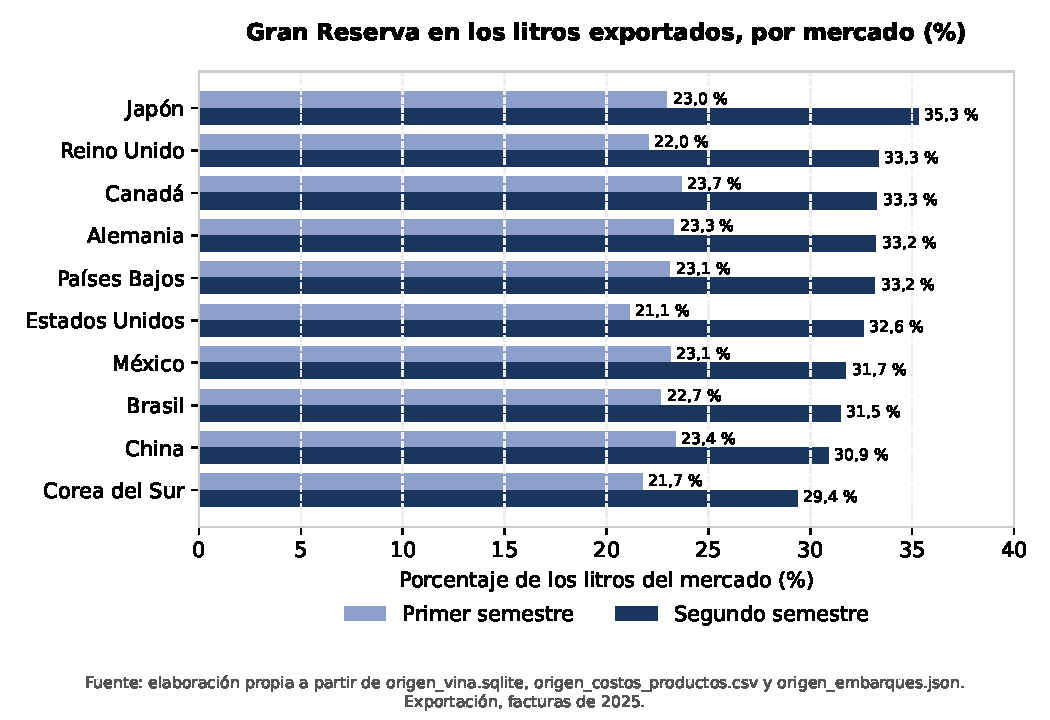
\includegraphics[width=0.58\linewidth]{figura4_gran_reserva_mercados.pdf}
  \caption{Participación de gran reserva en los litros, por mercado y semestre, \%. Fuente: elaboración propia sobre \texttt{fact\_venta}.}
  \label{fig:mercados}
\end{figure}

\noindent La figura respalda el supuesto S8: los diez mercados de exportación suben su participación de gran reserva entre el 1.\textsuperscript{er} y el 2.\textsuperscript{o} semestre, entre 7,5\,pp (China) y 12,3\,pp (Japón). Brasil, el único del hemisferio sur, sube 8,8\,pp.